\documentclass[10pt, oneside, titlepage]{ltjsarticle}  % bxjsarticleの代わりに

% 日本語フォント設定
\usepackage[haranoaji]{luatexja-preset}

% その他のパッケージは変更なし
\usepackage[margin=25truemm]{geometry}
\usepackage{graphicx}
% zxjatypeとzxjafontは削除
% \usepackage{zxjatype}
% \usepackage[ipaex]{zxjafont}

\usepackage{titling}
\usepackage{here}
\usepackage{ascmac}
\usepackage{amsmath}
\usepackage{amssymb}
\usepackage{ulem}
\usepackage{url}
\usepackage{mathtools}
\usepackage{float}
\usepackage{listings,jvlisting}

% Hyperref Setup
\usepackage[unicode,bookmarks=true,bookmarksnumbered=true,bookmarksopen=true,colorlinks=true,linkcolor=blue,urlcolor=blue]{hyperref}

% Custom Commands and Settings
\newcommand{\diff}{\mathrm{d}}
\def\qed{\hfill $\Box$}

% Listings Configuration
\lstset{
    basicstyle={\ttfamily},
    identifierstyle={\small},
    commentstyle={\small\itshape},
    keywordstyle={\small\bfseries},
    ndkeywordstyle={\small},
    stringstyle={\small\ttfamily},
    frame={tb},
    breaklines=true,
    columns=[l]{fullflexible},
    numbers=left,
    xrightmargin=0zw,
    xleftmargin=3zw,
    numberstyle={\scriptsize},
    stepnumber=1,
    numbersep=1zw,
    lineskip=-0.5ex
}

% Change "Listings" to "プログラム"
\renewcommand{\lstlistingname}{プログラム}

\title{ \large{2024A・機械情報冬学期演習・自主プロジェクト}\\
\vspace{1cm}
\Huge{卓球ロボット HARIMOTO}}
\author{東京大学工学部機械情報工学科3年 \\
学籍番号: 03-240281 \\
氏名: 椿 道智}

\begin{document}
\begin{titlepage}
  \begin{center}
  \Large{2024A・機械情報冬学期演習・自主プロジェクト}\\
  \vspace{1cm}
  \Huge{卓球ロボット HARIMOTO}\\
  \vspace{1cm}
  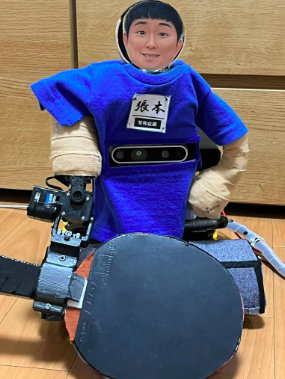
\includegraphics[width=10cm]{figures/HARIMOTO.png}\\
  \vspace{2cm}
  \Large{
  東京大学工学部機械情報工学科3年\\
  学籍番号: 03-240281\\
  氏名: 椿 道智
  }
  \end{center}
\end{titlepage}
\section{概要}
本プロジェクトでは,卓球台上を移動可能な卓球ロボット HARIMOTO(以下,単に「ロボット」という.)を製作した.ロボットは,「プッシュ卓球打ち(=温泉卓球打ち)」「ドライブ打ち」の二種類の打撃方法により,投げた卓球ボールに対して,タイミングを合わせてラケットを振ることができる.単に,打撃制御や画像処理をするだけではなく,ボールが返球された際の「チョレイ」効果音や外装の工夫により,実際の張本選手感(卓球選手感)を出し,ユーザ側が楽しめるようにも工夫した.

ソフトウェア面では,アームの動作(卓球ボールの打撃),D435iによる画像認識(卓球ボールの認識),ボールの着地予測,メカナムホイールの制御,音声再生を行った.機械工学少人数ゼミ(岡田慧教授ゼミ)や知能ロボット演習(機械情報冬学期演習)で学んだeuslisp・ROS noeticを用いてシステムを組んだ.

ハードウェア面では,4自由度アームの設計・製作,ラケットや服,左腕や靴など外装の製作・塗装を行った.

\section{動機・背景}
私は手術ロボットや医療ロボットに興味があり,特に縫合など針を使った自律的なタスクに関心がある.そのため,学期の初めには縫合ロボットを作ろうと考えていた.しかし,少人数ゼミで縫合に挑戦する機会が得られたため,自主プロジェクトではあえて全く異なるタスクのロボット製作に取り組むことにした.

自主プロジェクトは「何でも作っていい」という貴重な機会であるため,自分の趣味である卓球ロボットを作り,「自分が楽しむ」ことを最優先に考えた.卓球ロボットといえば,従来研究では卓球台の外に大きなパラレルリンクを設置して返球させる手法が主流なのは周知の通りである.しかし,似たようなものを作ってもオリジナリティがないと思い,本プロジェクトでは,従来の方法とは逆に「卓球台の上で省スペース」「シリアルリンク」の新しい卓球ロボットを制作することを目指した.

\section{コンセプト}
卓球選手の戦型は,前陣(速攻)型・中陣型・後陣型の3種類に大別される.それぞれ,卓球台のエンドラインから0mから1m離れた場所から打つ,1mから2m離れた場所から打つ,2m以上下がった場所から打つ戦型である.この内,前陣型は,卓球台にほとんどくっついて打つような戦型なので,ボールの着地直後にラケットをボールに接触させて返球させる.

前陣型の戦型が存在するということは,理論上は,(エッジボールなどを除いたほとんどのボールは),台から離れなくても「台上」で返球可能であり,この「前陣型」戦型が,私が今回「卓球台上」で返球するロボットが製作可能だと考えた根拠である.さらに,ほとんどのボールに対して着地直後の返球をするので,ラケットの存在する高さも低い範囲に制限できるというメリットがある.一方で,前陣「速攻」型とも言われるように,前陣でプレーをすることになると,ボールの返球までの時間的な猶予が少なくなり,素早い認識と判断が求められ,これが本プロジェクトの難点の1つにもなっている.

\section{環境構築・実行方法(Github)}
本プロジェクトにかかるすべてのソースコードと自作パーツのモデルは, \url{https://github.com/Michi-Tsubaki/ping-pong-robot}で公開している.
\begin{screen}
git clone https://github.com/Michi-Tsubaki/ping-pong-robot.git
\end{screen}

なお,本レポート内でも,説明に必要な範囲でソースコードを参照する.

\subsection{実行方法}
\begin{screen}
  cd ~/ping-pong-robot \\
  source devel/setup.bash \\
  roslaunch HARIMOTO all.launch \#画像処理やアームコントローラのノードを起動
\end{screen}
\begin{screen}
cd ~/ping-pong-robot\\
source devel/setup.bash \\
roscd HARIMOTO/src \\
emacs -nw 
M+x shell
source ~/ping-pong-robot/devel/setup.bash
roslaunch HARIMOTO all.launch \#画像処理やアームコントローラのノードを起動
\end{screen}
\section{機能}
ロボットは,以下の機能を備えている.
\begin{enumerate}
\item {\bf 着地予測して打つ} \\
 空間を「近距離」「中間距離」「遠距離」の3つの空間に分け,空間によって着地までの猶予が異なることから,前者から,予測せずに直ちに打つ,速度の生データから着地予測して打つ,速度にフィルタ処理を施して予測位置に移動して打つ,を機動的に使い分けながら打撃のタイミングを決めている.
\item {\bf 打つ→チョレイ} \\
 4自由度ながらも力強く打てるように試行錯誤した打撃関数を作成した(引数は高さ).上手く打てると,「チョレイ」と叫ぶ仕様にいなっている.
\item {\bf 打撃モード} \\
 開始時のアームの高さに応じて「プッシュ打ち」モードと「ドライブ打ち」モードを起動することができる.
\item {\bf 警告} \\
 サーボモータに長時間負荷をかけ続けると故障の原因となるため,起動後2分後と5分後に「腕が疲れてきたよ」という警告音を発し,プログラムの停止を促している.
\end{enumerate}
\section{システム構成}
ロボットのシステム構成は,図\ref{system}の通りである.ロボットは,4自由度ロボットアーム・Interl d435 depthカメラ・メカナムホイール・スピーカーから構成される.これらと,main.l(制御アルゴリズム),画像処理のノード(detect\_ball.launchで起動)をros topicでつなぐことでシステムが構成されている.詳細はros topicとros nodeのグラフ(rqtグラフ)を図\ref{rqt}に示すが,字が小さくて読みづらい.
\begin{figure}[H]
\centering
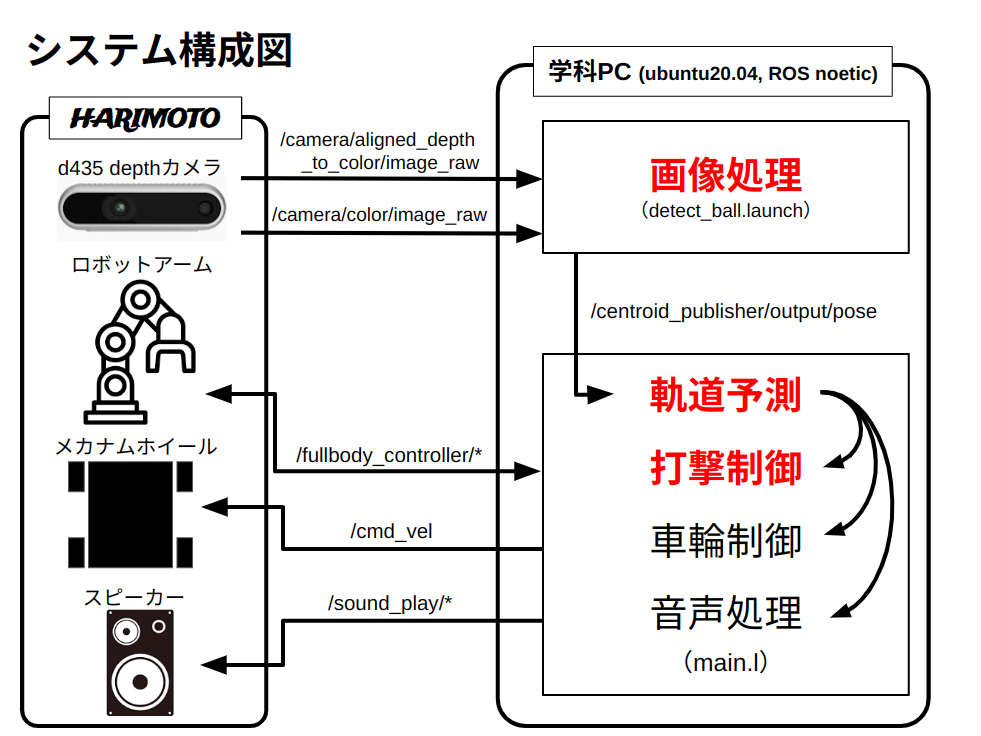
\includegraphics[width=12cm]{figures/system.png}
\caption{システム構成図}
\label{system}
\end{figure}
\begin{figure}[H]
\centering
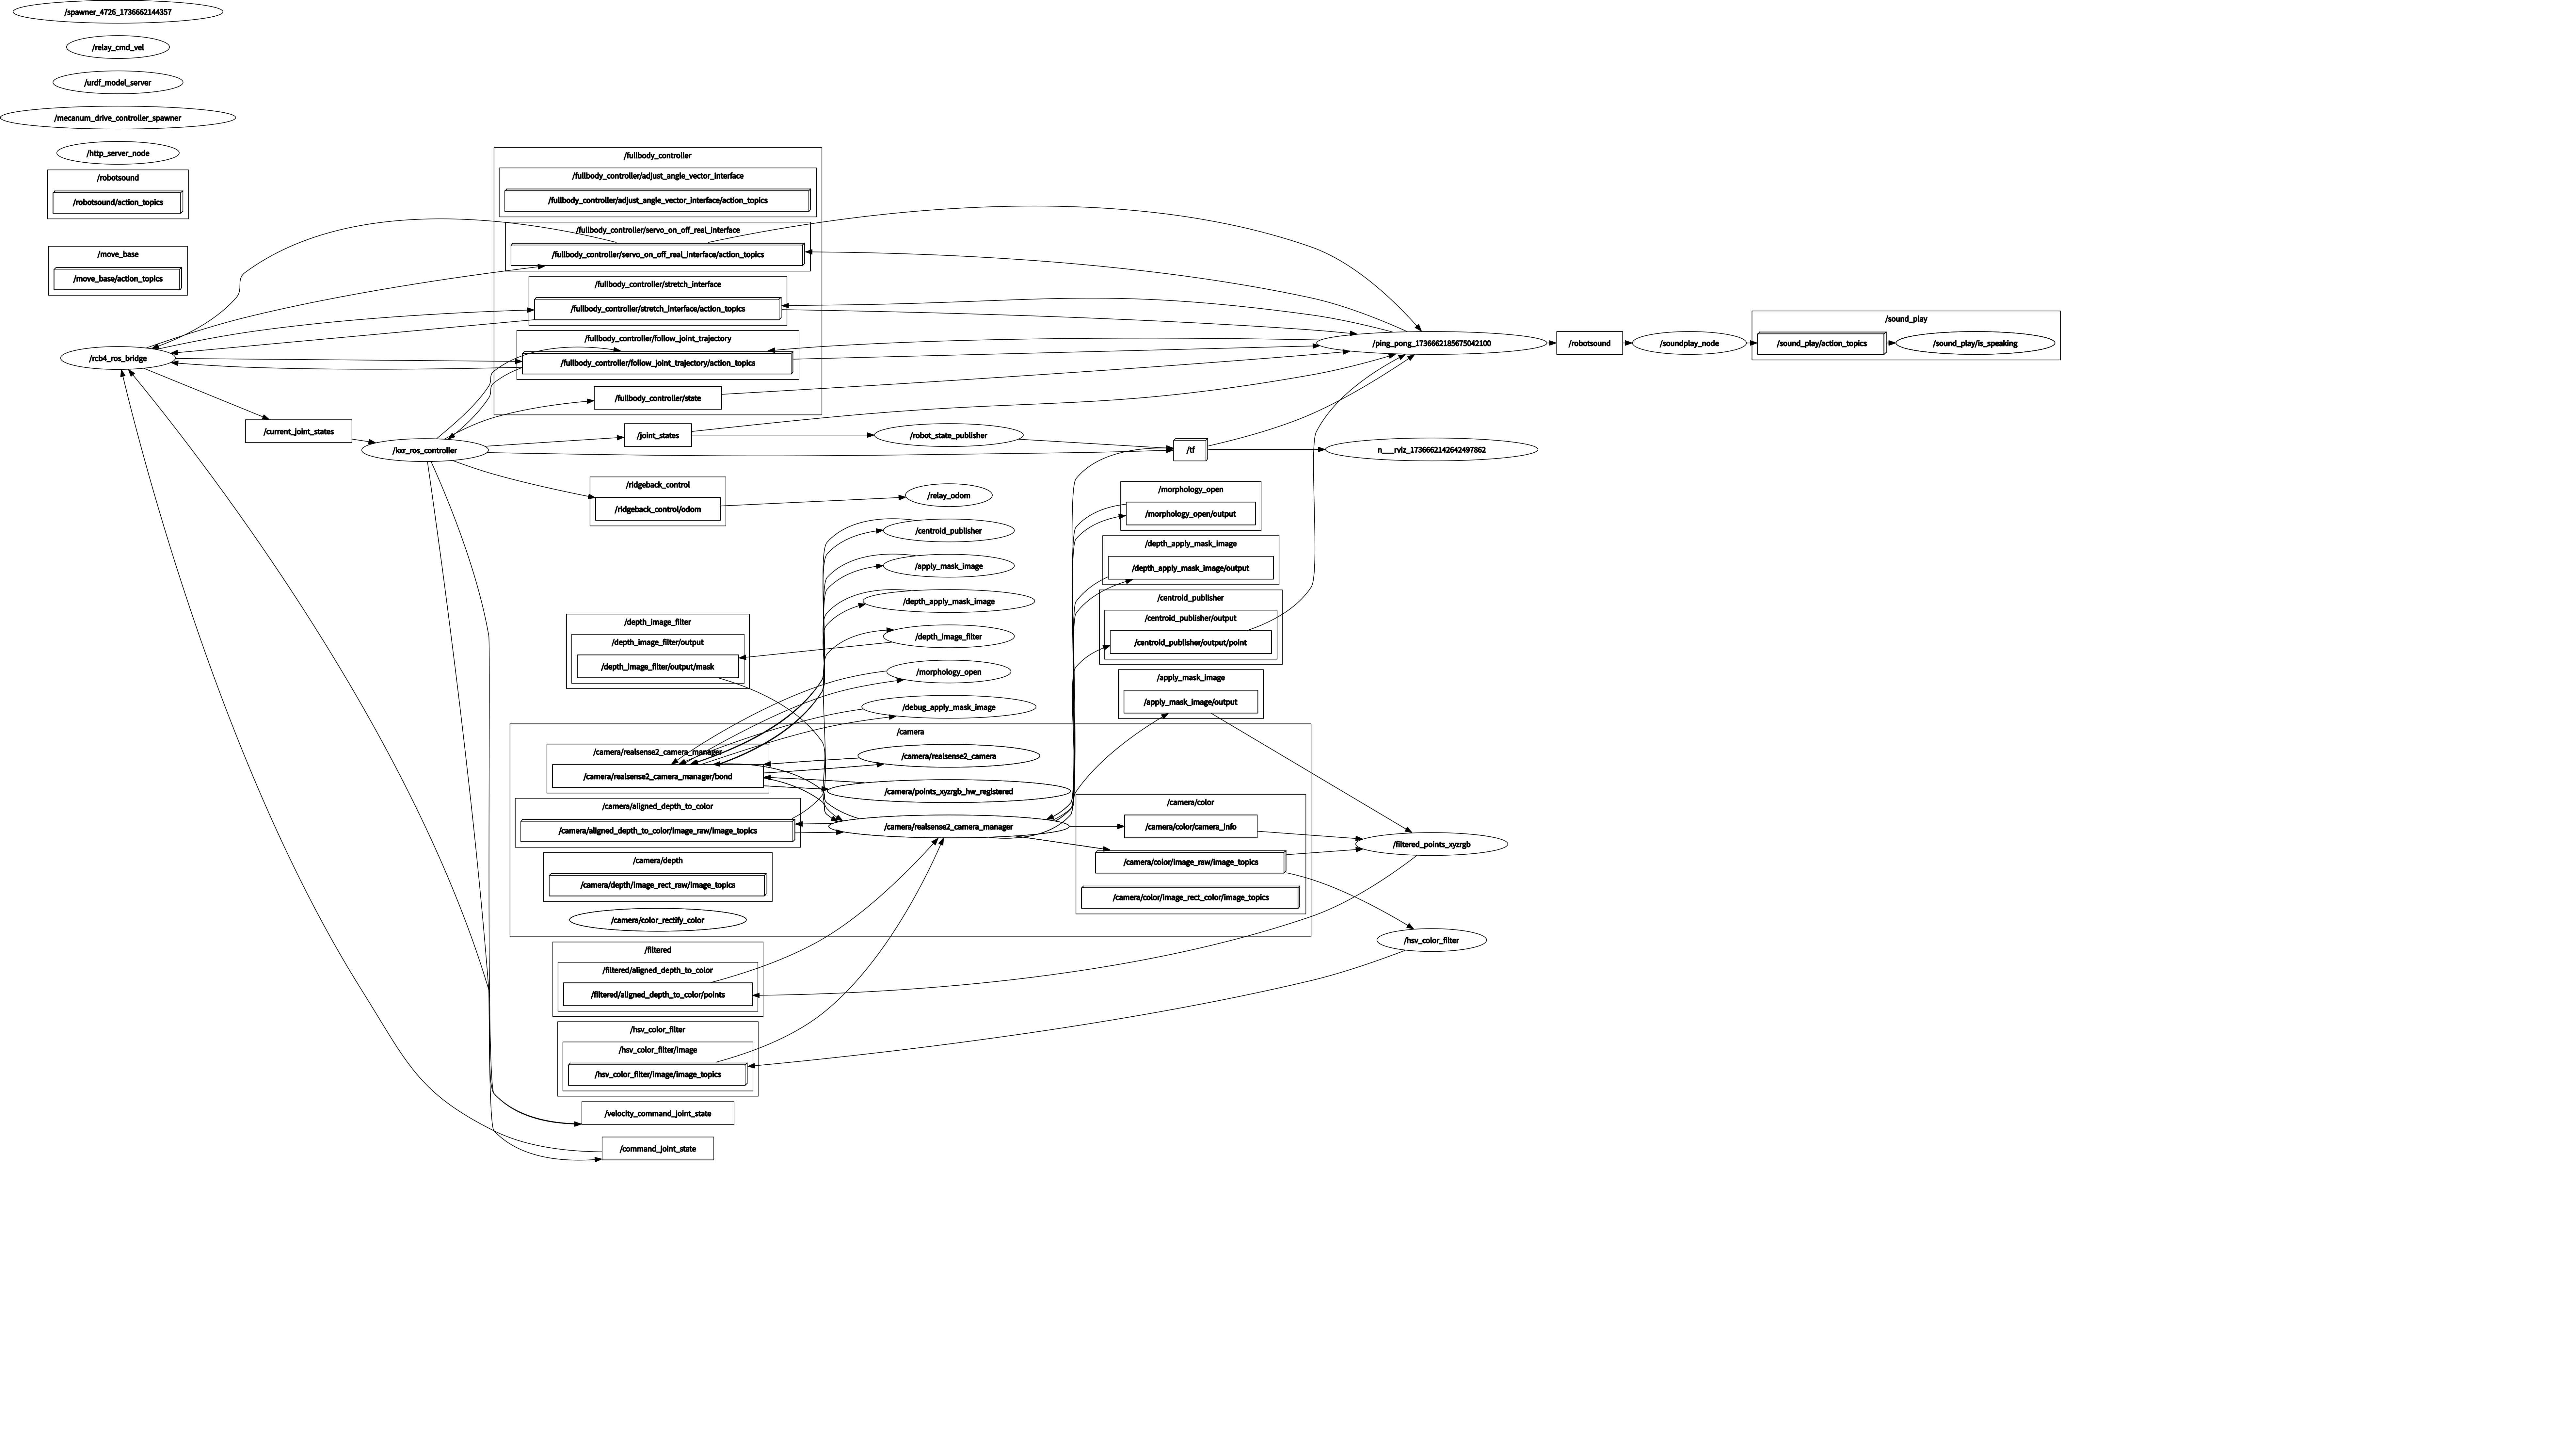
\includegraphics[width=15cm]{figures/rosgraph.png}
\caption{rqt\_graph}
\label{rqt}
\end{figure}
\section{ソフトウェア}
\subsection{統合制御アルゴリズム}
本節では,打撃(アーム)・軌道予測・画像認識・メカナム制御のサブルーチンを統合し,卓球ボールの返球を実現するアルゴリズムについて説明する.
\subsection{打撃}
本節では,卓球ロボットHARIMOTOの4軸ロボットアームによる打撃の方法について説明する.
\subsection{軌道予測}
\subsection{画像認識}
本節では,Intel RealSense Depth Camera D435iを用いたボールの中心位置の取得するプログラムついて説明する.
「HSVカラーフィルタ」で

苦労した点・新旧も含めて説明する.\cite{detect2}
\subsection{メカナムホイール制御}
本節では,メカナムホイールの制御プログラムについて説明する.
メカナムホイールの制御インタフェースはKXR ControllerとROS ControlのRidgeback Controllerを使用した.
この時点で
\begin{screen}
(send *ri* :send-cmd-vel-raw x y rot)
\end{screen}
を送ることで,cmd\_velに値をPublishすることができるようになった.

本プロジェクトでは,移動用のサブルーチンとして,基準値よりも左にいるか右にいるか,前にいるか後ろにいるかによって,逐次cmd\_velを送信する「move\_follow」関数と,指定した相対座標に移動する「move\_to」関数を実装した.
\begin{enumerate}
\item move\_follow \\
  ロボットが返球に対応できる範囲(sweet\_spot)に対して,逐次更新されるボールの着地予測地点がが右にあるか左にあるか,前にあるか後ろにあるかによって,逐次ロボットが動くことを目的としたサブルーチン.
  
\item move\_to \\
  camera\_link座標系(カメラに固定された座標)からの相対座標で計算されたボールの着地予想着地地点に直接移動することが可能.
\end{enumerate}
\cite{mecanum}
\subsection{音声再生}
本節では,音声に関する実装について説明する.\cite{sound}
\section{ロボットモデル・ハードウェア・メカニクス}
\subsection{ロボットモデル}
本節では,自作パーツを含むロボットのアセンブリからURDFの製作について説明する
\subsection{ロボット設計・製作}
本節では,ロボット全体の設計思想・製作,自作パーツの設計について説明する.

\subsection{外装}

\section{オリジナリティ・工夫}

\section{気づいたこと}




\section{作業記録(参考)}
本プロジェクトの進捗は,\url{http://github.com/Michi-Tsubaki/ping-pong-robot/issues}で管理した.詳細は,そちらを参照してほしい.ここでは,その要点を当初の計画と比較しながら振り返る.

\section{今後の展望}
本プロジェクトを始めた当初の目標は,大きな目標として,
\begin{enumerate}
  \item 来たボールを返球する
  \item ボールの着地予測地点に移動して返球する
  \item ボールの回転に応じて返球方法を動的に変えられるようにする
\end{enumerate}
の3点を掲げた.自主プロ発表会では,1.と2.を部分的ついて部分的に成功し発表することができた.一方で,
\begin{enumerate}
\item 返球できる確率は$\dfrac{1}{2}$程度に留まった
\item 移動して対応できる距離はせいぜい$\pm 10 cm$であり,それ以上は返球が間に合わないため狭い範囲に留まった
\item ドライブ打ちモードをコード上は実装したものの,動作パラメタのチューニングが間に合わなかった.また,プッシュ打ちとドライブ打ちを動的に変更するのは実現できなかった.
\end{enumerate}
は今後課題として残った.

ロボットを五月祭に展示するにあたり,春休みに以下の課題について調査・開発を行うことにした.
\subsection{画像認識:Depth情報のみからボールの位置を取得するアルゴリズムの開発}
D435iを用いたボールの位置判定を行う際,Depth情報を使用する前にカラーフィルターを用いたマスク処理をしている.そのため,ColorとDepthの両方の情報を同時に取得する必要があり,この場合の取得周期は「60fps」が限界である(両者が同期する必要があるため).この制約が位置取得の遅れのボトルネックとなり,返球できる確率を制限していると考えられる.

D435iは,Depth情報のみを使用する場合には300fpsを実現できるという公式の発表がある\cite{intel}.Depth情報だけを用いてボールの位置,速度,着地地点を予測するアルゴリズムを開発できれば,Color情報は不要となり,300fpsのフレーム情報を活用できるため,ラケットの振り遅れを大幅に減らし,返球確率を向上させることができると考えている.

Depth情報を処理する際にクラスタリングを行うと処理速度が遅くなることを,このプロジェクトを通じて痛感したため,クラスタリングを経由しないアルゴリズムを考案する必要がある.

以下は、本課題に対するアプローチで現時点で有用だと考えられるアプローチ(仮説)である.

\begin{itemize}
\item 深尾教授のロボットコントロールの講義で学んだ自動運転における「時間的に連続するフレームの差分を取ることで移動する障害物(人など)の情報を抽出する」手法を応用することで,移動物体であるボールを効率的に検出できるのではないかと考えている.時間計算量は処理で扱う点数(特徴点の数)に依存するため,この特徴点抽出により処理全体が高速化できると予想している.

\item 國吉教授のロボットインテリジェンスの講義で学んだ「Time to Collision(衝突までの時間)」の概念を用いることで,ボールの着地予測時間を簡単に算出でき,計算処理の高速化が期待できる.

\item 矢野倉先生から助言をいただいた「半円殻(卓球ボールの像)」のマッチングや,岡田ゼミで使用した「Hough変換による円抽出」を3次元空間に応用する方法(射影処理など)を通じて,ボールを抽出する手法を取り入れたいと考えている.
\end{itemize}

この春休みを通じて,上記の仮説を検証し,計算量を削減するための特徴点抽出とDepthフレームからの卓球ボール検出をの課題に取り組んでいく.



\subsection{ドライブ打ちモードのパラメタチューニング}
前述したとおり,ドライブモードをできるシステム構成は完成しているので,ロボットアームの初期姿勢やラケットを振るアームの速度・経路を調整する.また,ボールがこの範囲に着地するときにラケットを振るというしきい値もプッシュ打ちモードとは異なるはずなので,その範囲(スイートスポットの値など)も調整する.

\section{謝辞}
本プロジェクトに取り組むに際し,ラフスケッチ・詳細スケッチに対して実現可能性や計画性,機構面で改善すべき点についてアドバイスをくださった小島邦生先生,Depth Cameraによる画像処理の方法やKXRのConfigurationについての逐次の質問やロボットパーツなどの資材の貸出対応で大変お世話になった矢野倉伊織先生,3Dプリンタ環境をご提供くださったメカノデザイン工房の技術職員の方々,アドバイスをくれた機械情報工学科の同級生に御礼申し上げます.

\begin{thebibliography}{9}
\bibitem{detect2} 
Michi-Tsubaki, ``recognize\_wound.launch,'' jsk\_demosm GitHub. [Online]. Available: 
\path{https://github.com/Michi-Tsubaki/jsk_demos/blob/jsk_2024_10_semi/jsk_2024_10_semi/pr2_surgery/launch/recognize_wound.launch}

\bibitem{mecanum} 
iory, ``[jedy\_bringup] support mecanum drive using ridgeback\_control \#2,'' robot-programming, GitHub. [Online]. Available: 
\path{https://github.com/iory/robot-programming/pull/2}

\bibitem{sound} 
jsk-ros-pkg, ``speak.l,'' jsk\_pr2eus, GitHub. [Online]. Available: 
\path{https://github.com/jsk-ros-pkg/jsk_pr2eus/blob/master/pr2eus/speak.l}

\bibitem{intel}
intel realsense, ''High Speed Capture for Intel® RealSense™ Depth Cameras'', April 8, 2020,
\path{https://www.intelrealsense.com/high-speed-mode-at-300-fps-for-depth-camera/}
\end{thebibliography}

\end{document}
